%\pagebreak
\noindent \underline{\textbf{Medan Listrik}}
\vskip 10pt
\begin{enumerate}
    \item \underline{\textbf{Elektron Bergerak Parabola dalam Pengaruh Medan Listrik}}
    \vskip5pt
    Suatu elektron ditembakkan dengan kecepatan awal $v_0$ dan dengan sudut elevasi $\theta$. Jarak kedua keping $d$ dan panjang keping $L$. Jika $v_0 = 5.83\times 10^6 m/s$ dan $\theta = 39^{\circ} ; E= 1870N/C$ (arah keatas), $d=1.97cm$ dan $L=6.20 cm$. Elektron akan menumbuk keping atas atau keping bawah? Dimana?

    \begin{center}
    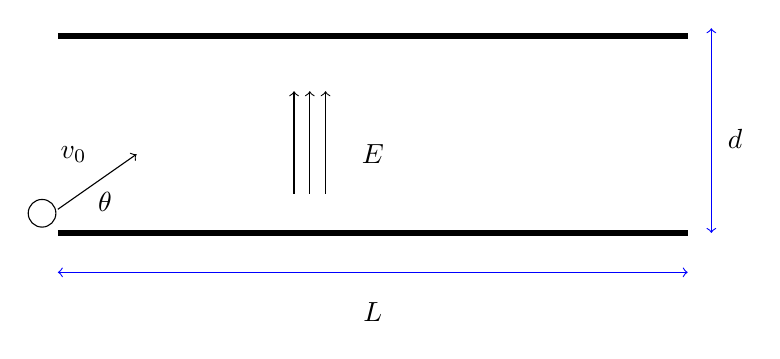
\begin{tikzpicture}
    	\draw [line width=2pt](0,0) -- (8,0);
    	\draw [line width=2pt](0,2.5) -- (8,2.5);
        \draw [->](3,0.5)--(3,1.8);
        \draw [->](3.2,0.5)--(3.2,1.8);
        \draw [->](3.4,0.5)--(3.4,1.8);
        \draw [->](0,0.3)--(1,1);
        \draw (-0.2,0.25) circle [radius=5pt];
        \draw [<->,blue] (0,-0.5)--(8,-0.5);
        \draw [<->,blue] (8.3,0)--(8.3,2.6);
        \node at (4,1) {$E$};
        \node at (0.6,0.4) {$\theta$};
        \node at (0.2,1){$v_0$};
        \node at (4,-1) {$L$};
        \node at (8.6,1.2){$d$};
    \end{tikzpicture}
    \end{center} 
    \pagebreak
    Medan listrik mengarah ke atas maka plat bawah bermuatan positif dan plat atas bermuatan negatif. Elektron akan bergerak parabola dimana selama pergerakannya mengalami percepatan kearah bawah karena elektron akan tertarik menuju plat bawah yang bermuatan positif.\\
    \begin{center}
    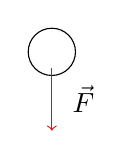
\begin{tikzpicture}
        \draw (0,0) circle [radius=3mm];
        \draw[red,->](0,-0.2)--(0,-1);
        \node at (0.4,-0.6) {$\vec{F}$};
    \end{tikzpicture}
    \end{center}
    Percepatan yang dialami elektron
    \begin{align*}
        \sum \vec{F}=m\vec{a}\\
        q\vec{E}=m\vec{a}\\
        -eE(\hat{i})=m\vec{a}\\
        \vec{a}=-\frac{eE}{m}\hat{i}
    \end{align*}
    Hitung ketinggian maksimum. Jika $y>d$ maka elektron menumbuk plat atas dan sebaliknya jika $y<d$ elektron menumbuk plat bawah.

    Waktu elektron sampai ketinggian maksimum
    \begin{align*}
        v=v_{0y}+at\\
        0=v_{0}sin\theta-\frac{eE}{m}t\\
        t =\frac{m}{eE}v_{0}sin\theta
    \end{align*}

    Ketinggian maksimum
    \begin{align*}
        y&=y_{0}+v_{0y}t+\frac{1}{2}at^{2}\\
        &=y_{0}+v_{0}sin\theta \cdot t-\frac{1}{2}\frac{eE}{m}t^{2}\\
        &=0+v_{0}sin\theta \cdot t-\frac{1}{2}\frac{eE}{m}t^{2}\\
        &=v_{0}sin\theta \left ( \frac{m}{eE}v_{0}sin\theta \right )-\frac{1}{2}\frac{eE}{m}\left ( \frac{m}{eE}v_{0}sin\theta \right )^{2}\\
        &=\left (\frac{m}{eE}v_{0}^{2}sin^{2}\theta\right )-\frac{1}{2}\left ( \frac{m}{eE}v_{0}^{2}sin^{2}\theta \right )\\
        &=\frac{m}{2eE}v_{0}^{2}sin^{2}\theta\\
        &=\frac{9.11\times 10^{-31}}{2\cdot 1.6\times 10^{-19}\cdot 1870}\left ( 5.83\times10^{6} \right )^{2}sin^{2}39^{\circ}\\
        y&=0.0205m\\
        y&=2.05cm
    \end{align*}
        Karena $y>d$ maka elektron menumbuk plat atas. Selanjutnya hitung waktu elektron menumbuk plat atas (pada ketinggian $d$) kemudian dapat dihitung pula jarak tempuh pada arah horizontal.
    \begin{align*}
        y&=y_{0}+v_{0y}t+\frac{1}{2}at^{2}\\
        d&= 0 +v_{0}sin\theta\cdot t-\frac{1}{2}\frac{eE}{m}\cdot t^{2}\\
        1.97\times10^{-2}&=3.66\times 10^{6}\cdot t-1.64\times 10^{14}\cdot t^{2}\\
        &1.64\times 10^{14}\cdot t^{2}-3.66\times 10^{6}\cdot t+1.97\times10^{-2}=0\\
        t&=\frac{-(-3.66\times 10^{6})\pm \sqrt{(-3.66\times 10^{6})^{2}-(4\cdot 1.64\times 10^{14}\cdot 1.97\times10^{-2})}}{2\cdot 1.64\times 10^{14}}\\
        t&=(1.115\times10^{-8})\pm (2.09\times10^{-9})
    \end{align*}
    Karena elektron bergerak parabola, maka elektron (jika tidak ada plat) dapat mencapai ketinggian $d$ sebanyak 2 kali. Karena ada plat atas, maka waktu yang dipilih adalah waktu yang pertama (simbol negatif) sehingga 
    \begin{align*}
        t&=(1.115\times10^{-8})- (2.09\times10^{-9})\\
        t&=9.06\times10^{-9}s
    \end{align*}
    Posisi horizontal elektron menumbuk plat atas
    \begin{align*}
        x&=v_{0x}t\\
        &=v_{0}cos\theta\cdot t\\
        &=(5.83\times 10^{6})cos(39)^{\circ}\cdot 9.06\times10^{-9}\\
        &=0.041m\\
        &\fbox{$x\approx4.1cm$}
    \end{align*}

% == 

    \begin{minipage}{0.6\textwidth}
    \item \underline{\textbf{Kesetimbangan Bandul Bermuatan}}
    \vskip5pt
    Suatu bola bermassa $m$ digantungkan dengan sutas tali pada suatu bidang bermuatan yang terdistribusi merata (non-konduktor). Bola bermuatan $q$ dan bola seimbang ketika tali membentuk sudut $\theta$ bidang dengan vertikal. Hitung kerapatan muatan bidang!
    \end{minipage}
    \hfill
    \begin{minipage}{0.25\textwidth}
    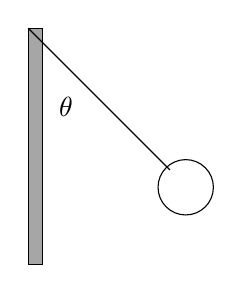
\begin{tikzpicture}
        \filldraw[fill=gray!70] (0,0) rectangle (0.18,3);
        \draw (1.8,1.2)--(0,3);
        \draw (2,0.98) circle [radius=10pt];
        \node at (0.48,2) {$\theta$};
    \end{tikzpicture}
    \end{minipage}

    \begin{center}
    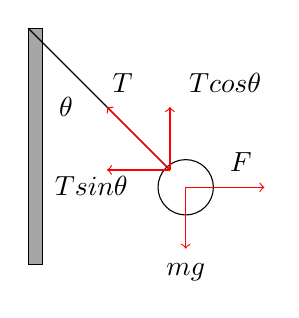
\begin{tikzpicture}
        \filldraw[fill=gray!70] (0,0) rectangle (0.18,3);
        \draw (1.8,1.2)--(0,3);
        \draw (2,0.98) circle [radius=10pt];
        \node at (0.48,2) {$\theta$};
        \draw [red,->] (1.8,1.2)--(1,2);
        \draw [red,->] (1.8,1.2)--(1.8,2);
        \draw [red,->] (1.8,1.2)--(1,1.2);
        \node at (1.2,2.3){$T$};
        \node at (2.5,2.3){$Tcos\theta$};
        \node at (0.8,1){$Tsin\theta$};
        \draw [red,->] (2,0.98)--(2,0.2);
        \node at (2,-0.1){$mg$};
        \draw [red,->] (2,0.98)--(3,0.98);
        \node at (2.7,1.3){$F$};
    \end{tikzpicture}
    \end{center}

    Sistem pada keadaan setimbang
    \vskip5pt
    \begin{minipage}{0.3\textwidth}
    \begin{align*}
        \sum F_{x}&=0\\
        F-Tsin\theta&=0 \\
        F&=Tsin\theta \\
        qE &= Tsin\theta \hskip10pt (1)
    \end{align*}
    \end{minipage}
    \hfill
    \begin{minipage}{0.3\textwidth}
    \begin{align*}
        \sum F_{y}&=0\\
        Tcos\theta-mg&=0\\
        Tcos\theta&=mg \hskip10pt (2)
    \end{align*}
    \end{minipage}
    \hfill
    \begin{minipage}{0.3\textwidth}
    \begin{align*}
        \frac{Tsin\theta}{Tcos\theta}&=\frac{qE}{mg}\\
        tan\theta&=\frac{qE}{mg} \hskip10pt (3)
    \end{align*}
    \end{minipage}
    
    \pagebreak
    \begin{minipage}{0.3\textwidth}
    \vskip5pt
    \begin{center}
    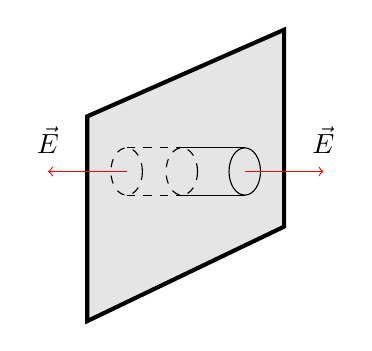
\begin{tikzpicture}
        \filldraw[fill=gray!20,line width=1.5pt] (0,-0.1)--(2.5,1)--(2.5,-1.5)--(0,-2.7)--cycle;
        \draw (2,-0.8) ellipse (0.2 and 0.3);
        \draw [dashed](0.5,-0.8) ellipse (0.2 and 0.3);
        \draw [dashed](1.2,-0.8) ellipse (0.2 and 0.3);
        \draw (1.2,-0.5) -- (2,-0.5);
        \draw (1.2,-1.1) -- (2,-1.1);
        \draw [dashed](0.5,-0.5)--(1.2,-0.5);
        \draw [dashed](0.5,-1.1) -- (1.2,-1.1);
        \draw [red,->](2,-0.8)--(3,-0.8);
        \draw [red,->](0.5,-0.8)--(-0.5,-0.8);
        \node at (3,-0.4){$\vec{E}$};
        \node at (-0.5,-0.4){$\vec{E}$};
    \end{tikzpicture}
    \end{center}
    \end{minipage}
    \hfill
    \begin{minipage}{0.3\textwidth}
    Gunakan Hukum Gauss
    \begin{align*}
        \oint \vec{E}\cdot\vec{dA}&=\frac{q}{\varepsilon_{0}}\\
        2E\cdot A&=\frac{q}{\varepsilon_{0}}\\
        E&=\frac{q}{2A\varepsilon_{0}}\\
        E&=\frac{\sigma}{2\varepsilon_{0}}\hskip10pt (4)
    \end{align*}    
    \end{minipage}
    \hfill
    \begin{minipage}{0.3\textwidth}
    Substitusi $(4)$ ke $(3)$
    \begin{align*}
        tan\theta&=\frac{qE}{mg} \\
        tan\theta&=\frac{q}{mg}\frac{\sigma}{2\varepsilon_{0}}\\
        &\fbox{$\sigma = \frac{2mg\varepsilon_{0}tan\theta}{q}$}
    \end{align*}    
    \end{minipage}

    \item \underline{\textbf{Perlambatan Elektron Oleh Plat Bermuatan}}
    \vskip5pt 
    Suatu elektron $115keV$ ditembakkan ke arah suatu lembaran plastik yang mempunyai kerapatan permukaan $-2.08\mu C/m^{2}$. Dari jarak berapa elektron harus ditembakkan agar kecepatan saat menyentuh lembaran itu nol?

    \begin{minipage}{0.5\textwidth}
    \begin{center}
    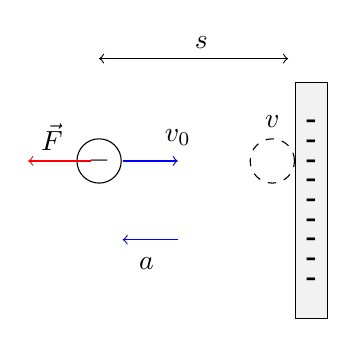
\begin{tikzpicture}
        \draw (0,0) circle [radius=8pt];
        \draw [dashed](2.2,0) circle [radius=8pt];
        \node at (0,0){$-$};
        \filldraw [fill=gray!10] (2.5,1) rectangle (2.9,-2);
        \foreach \x in {1,0.5,...,-3}{
        \node at (2.7,\x*0.5) {\textbf{-}};
        }
        \draw [<->] (0,1.3)--(2.4,1.3);
        \node at (1.3,1.5){$s$};
        \draw [blue,->] (0.3,0)--(1,0);
        \node at (1,0.3){$v_{0}$};
        \node at (2.2,0.5){$v$};
        \draw [blue,<-] (0.3,-1)--(1,-1);
        \node at (0.6,-1.3){$a$};
        \draw [red,->] (-0.1,0)--(-0.9,0);
        \node at (-0.6,0.3){$\vec{F}$};
    \end{tikzpicture}
    \end{center}
    \end{minipage}
    \hfill
    \begin{minipage}{0.4\textwidth}
    \begin{align*}
        E_{k}&=115keV\\
            &= 115(10^{3})(1.6\times10^{-19})\\
            &= 1.84\times 10^{-14}J\\
        \sigma&=-2.08\mu C/m^{2}\\
        &= -2.08\times 10^{-6}C/m^{2}
    \end{align*}
    \end{minipage}
    \vskip5pt
    Elektron (bermuatan negatif) mendekati plat yang memiliki rapat muatan negatif. Karena muatan sejenis (tolak menolak), elektron lama kelamaan akan diperlambat hingga berhenti ketika menyentuh plat. 

    \begin{minipage}{0.4\textwidth}
    \begin{align*}
        \vec{E}&=\frac{\sigma}{2\varepsilon_{0}}\\
        \frac{\vec{F}}{q}&=\frac{\sigma}{2\varepsilon_{0}}\\
        -ma&=\frac{q\sigma}{2\varepsilon_{0}}\\  
    \end{align*}
    \end{minipage}
    \hfill
    \begin{minipage}{0.5\textwidth}
    \begin{align*}
        a&=-\frac{-e\sigma}{2m\varepsilon_{0}}\\
        a&= -\frac{(-1.6\times10^{-19})(-2.08\times 10^{-6})}{2(9.11\times10^{-31})(8.85\times10^{-12})}\\
        a &= -2.06\times10^{16}m/s^{2}
    \end{align*}
    \end{minipage}
    Gunakan persamaan GLBB untuk menghitung jarak elektron ketika mula-mula ditembakkan
    
    \begin{minipage}{0.5\textwidth}
    \begin{align*}
        E_{k}&=\frac{1}{2}mv_{0}^{2}\\
        v_{0}^{2}&=\frac{2E_{k}}{m}\\
        &=\frac{2\cdot1.84\times10^{-14}}{9.11\times10^{-31}}\\
        &= 4.03\times10^{16}(m/s)^{2}
    \end{align*}
    \end{minipage}
    \hfill
    \begin{minipage}{0.5\textwidth}
    \begin{align*}
        v^{2}&=v_{0}^{2}+2as\\
        0 &= (4.03\times10^{16})+2(-2.06\times10^{16})s\\
        s &= \frac{4.03\times10^{16}}{2\cdot2.06\times10^{16}}\\
        s &= 0.978 m\\
        &\fbox{$s = 97.8cm$}
    \end{align*}
    \end{minipage}
    
\end{enumerate}
